\documentclass[a4paper, 12pt]{extarticle}
\usepackage[english, russian]{babel}
\usepackage[utf8x]{inputenc}
\usepackage{fullpage}
\usepackage{indentfirst} % Первый абзац в разделе тоже с красной строки
\usepackage{cmap} % для кодировки шрифтов в pdf (чтобы не было крокозябры при копировании из pdf )
\usepackage{graphicx} % для вставки картинок
\sloppy % Включение переноса слов в тексте

\usepackage{hyperref} % Для добавления ссылок в тесте

% Настройка цветов для ссылок
\hypersetup{
colorlinks = true,
linkcolor = black,
pagecolor = black,
urlcolor = blue, 
citecolor = black
}

\usepackage[labelfont=bf, labelsep=space]{caption} % Делаем надписи "Рис.1" под рисунками жирными и без двоеточия.

\usepackage[top=20mm, bottom=20mm, left=20mm, right=20mm
, nohead % Убрать расстояние для верхних колонтикулов
%, nofoot % Убрать расстояние для нижних колонтикулов
]
{geometry} % Размер полей у старницы
\setlength{\parindent}{1.25cm} % Размер интервала для абзацев 
\usepackage{setspace}
\onehalfspacing % одинарный интервал

\usepackage{caption} % подписи к рисункам в русской типографской традиции
\DeclareCaptionFormat{GOSTtable}{#2#1\\#3\vspace*{-\baselineskip}}
\DeclareCaptionLabelSeparator{fill}{\hfill}
\DeclareCaptionLabelFormat{fullparents}{\bothIfFirst{#1}{~}#2}
\captionsetup[table]{
     format=GOSTtable,
     %font={footnotesize},
     labelformat=fullparents,
     labelsep=fill,
     labelfont=normal,
     textfont=bf,
     justification=centering,
     singlelinecheck=false
     }

\begin{document}
\section*{Маршрут до места проведения посвята}
\subsection*{Общий вид}
\par Маршрут проложен от Красной площади до места проведения посвята. Сам маршрут Вы можете видеть на рисунке~\ref{ris:generalRoute}. Протяженность маршрута около 20 км, время без пробок 39 минут. Дорога за городом столь убога, что 40 минут светит только внедорожнику. Рассчитывайте время с запасом.

\par Если кто-то хочет самостоятельно построить себе маршрут, то вот примерные координаты для Яндекса 57.541585, 39.700436. В принципе эти же координаты работают на картах от Google. Более того у Google есть StreetView практически на весь маршрут движения. Очень рекомендую им воспользоваться.
\begin{figure}[h!]
	\center{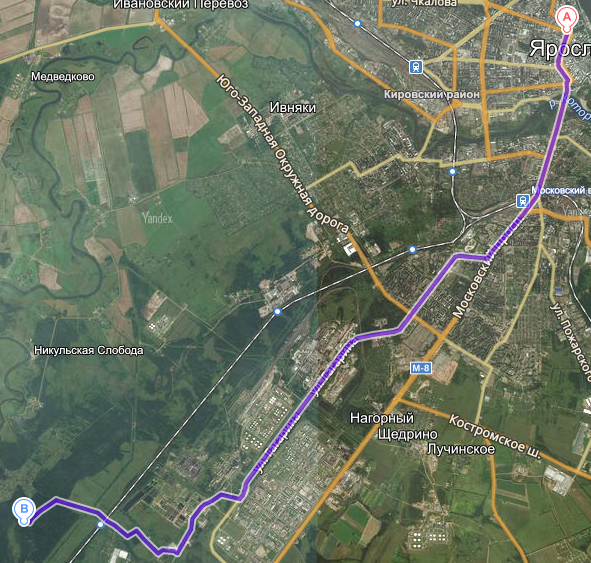
\includegraphics[width=0.9\linewidth]{YandexMap}}
	\caption{Общий вид маршрута}
	\label{ris:generalRoute}
\end{figure}

\newpage
\subsection*{Детализация проезда}
\par Первый ориентир на пути к посвяту --- улица Гагарина. По ней нужно ехать реально очень долго, фактически до её конца. Необходимо добраться до проходных НПЗ, точка B на карте (см. рис~\ref{ris:generalRoute}). Для это нужно просто ехать прямо. Не сворачивать никуда. Даже если Вам и Вашей спутнице кажется, что настало время повернуть. Даже если вы в один голос орете, что узнаете место и вам туда. Нет, вам до проходных(см. рис~\ref{ris:NPZ}).
\begin{figure}[h!]
	\center{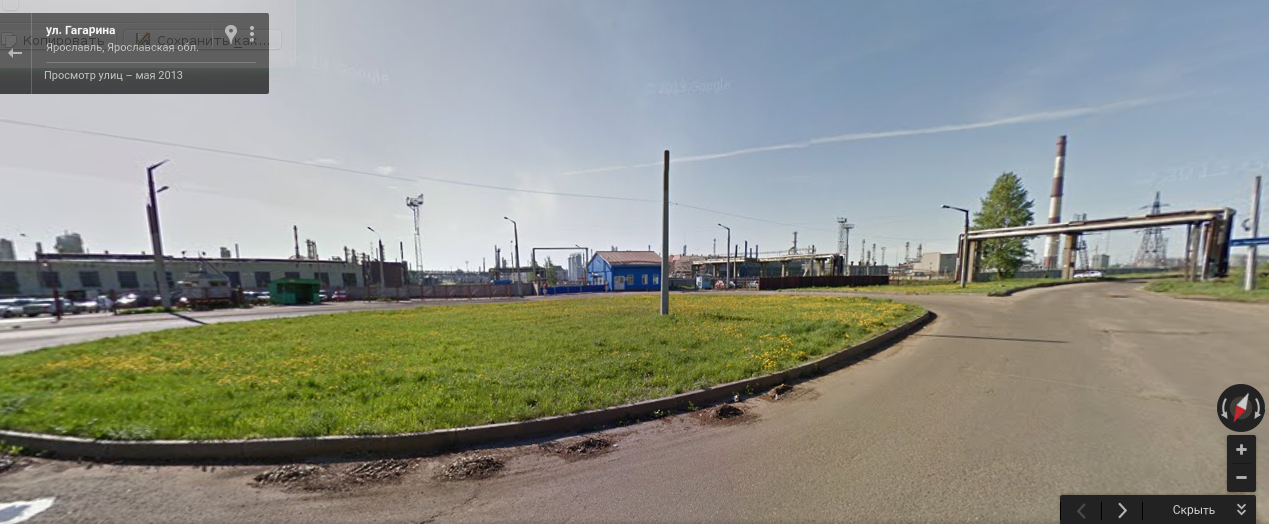
\includegraphics[width=0.9\linewidth]{NPZ}}
	\center{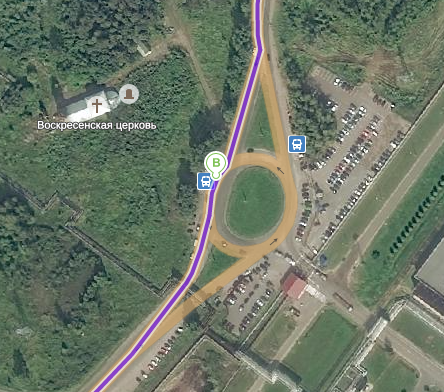
\includegraphics[width=0.65\linewidth]{npzMap}}
	\caption{Проходные НПЗ}
	\label{ris:NPZ}
\end{figure}

\par Затем нужно проехать немного прямо (под трубами, которые видно на рисунке~\ref{ris:NPZ}) и повернуть направо, точка C на карте. Фактически продолжая движение по улице Гагарина, там даже указатель на фото есть, вроде был он и в жизни (см. рис~\ref{ris:afterNPZ}).
\begin{figure}[h!]
	\center{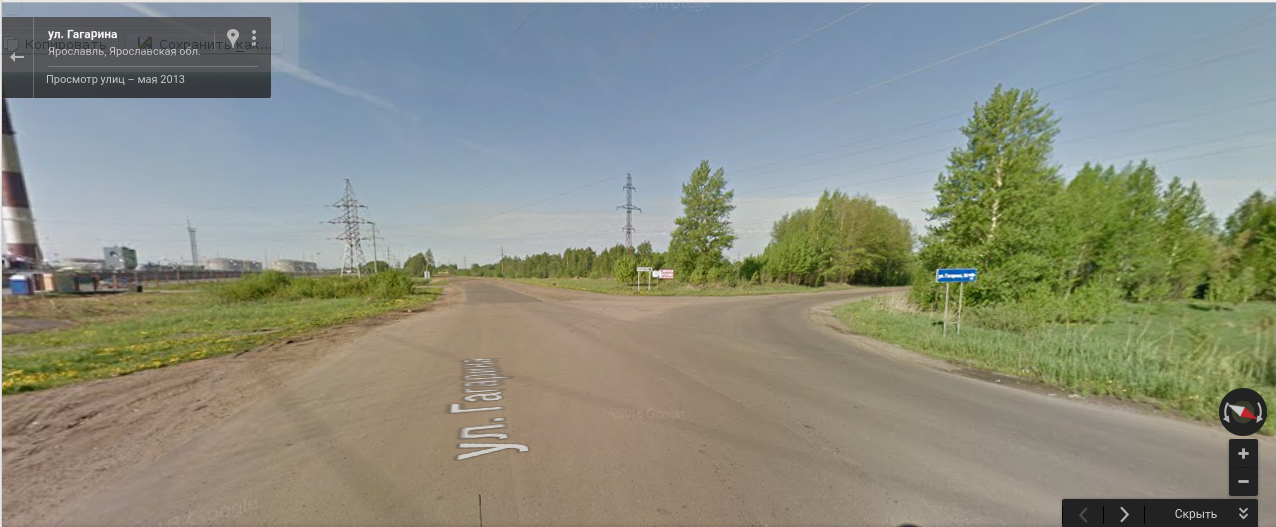
\includegraphics[width=0.9\linewidth]{afterNPZ}}
	\center{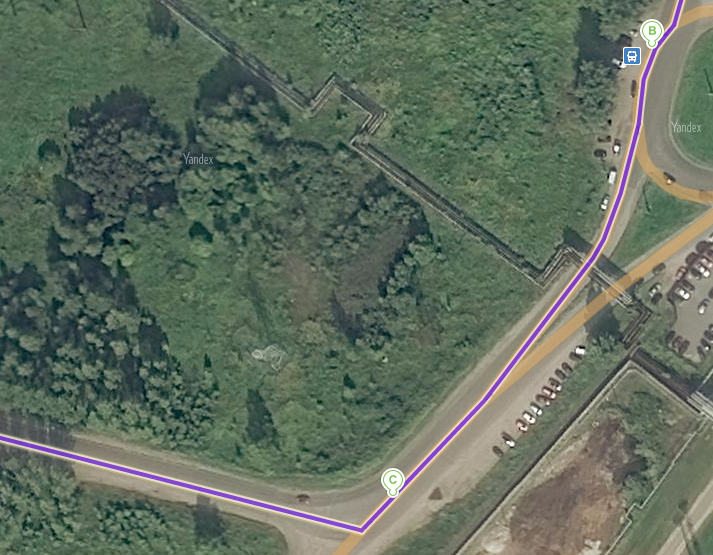
\includegraphics[width=0.65\linewidth]{afterNPZMap}}
	\caption{Поворот направо после проходных}
	\label{ris:afterNPZ}
\end{figure}

\par Теперь необходимо просто ехать по этой <<дороге>> некоторое время. Очень важно не повернуть слишком рано, но рецепта как удержать себя на этой дороге у меня нет. Нужно доехать до забора (см. рис~\ref{ris:zabor}), точка D. Будет одно очень спорное место: поворот направо и небольшой пригорок --- Вам на пригорок. Осознанно не указываю это место на карте, чтобы не сбивать с верного пути лишними отметками. При удачном раскладе у этого самого забора необходимо повернуть направо и продолжать движение. Дорога там одна, как минимум я так помню.
\begin{figure}[h!]
	\center{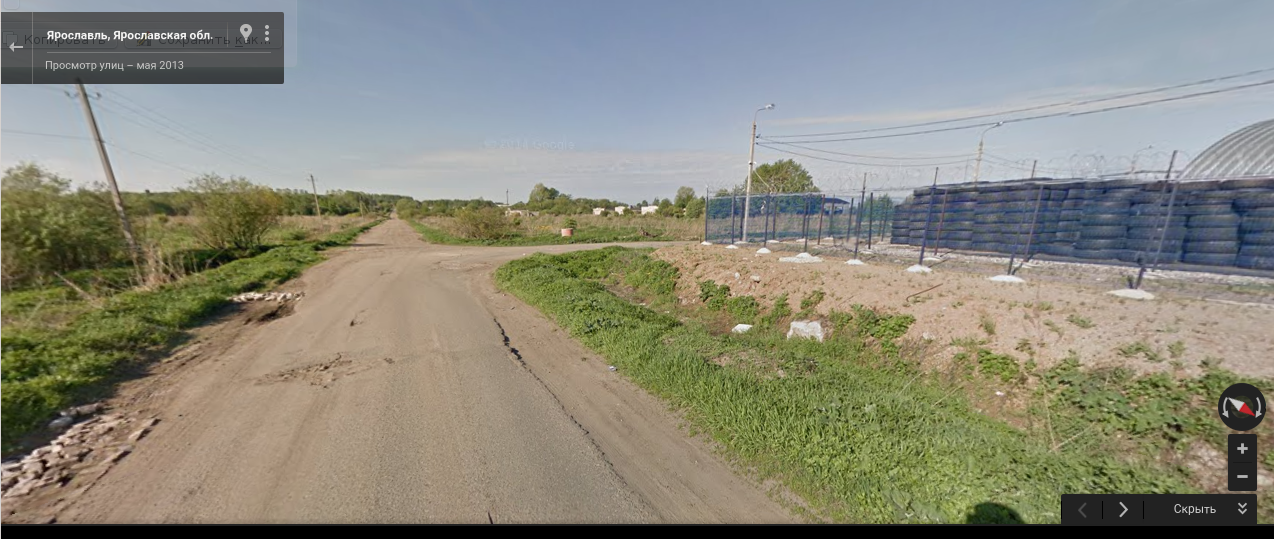
\includegraphics[width=0.9\linewidth]{zabor}}
	\center{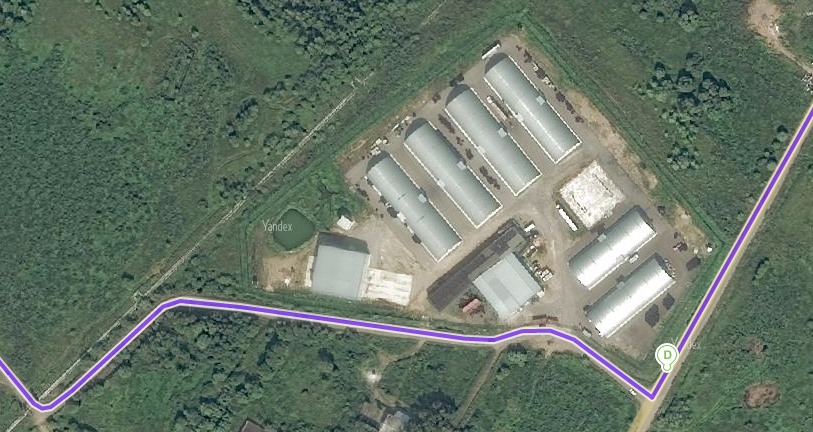
\includegraphics[width=0.65\linewidth]{zaborMap}}
	\caption{Забор}
	\label{ris:zabor}
\end{figure}

\par Через некоторое время Вы доедете до переезда через железную дорогу, там еще и станция недалеко (если есть герои, которые отважатся ехать на посвят на электричке; прецеденты были). Обращу внимание что Яндекс и Google несколько расходятся в названиях станции, но географически место одно и то же. Если верить картам, то после переезда нет поворотов налево, кроме нужного. Как он выглядит можно увидеть на рисунке~\ref{ris:last}, точка E.
\begin{figure}[h!]
	\center{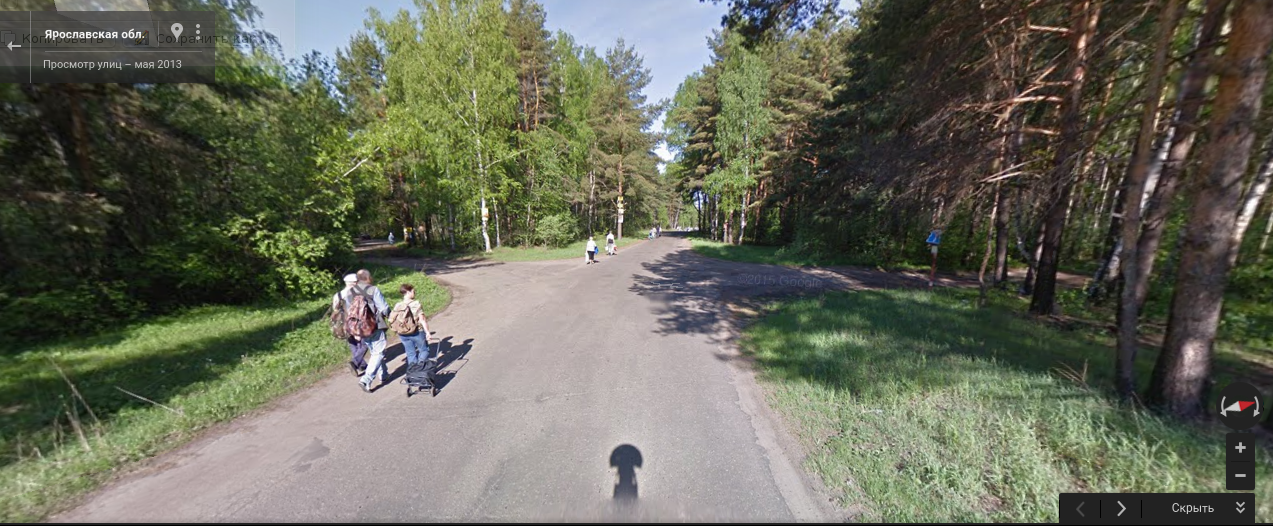
\includegraphics[width=0.9\linewidth]{last}}
	\center{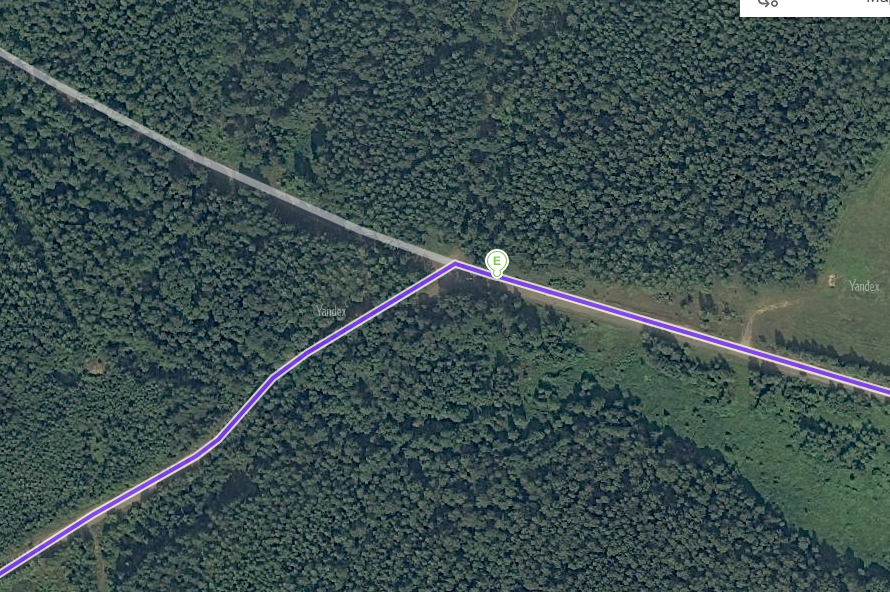
\includegraphics[width=0.5\linewidth]{lastMap}}
	\caption{Последняя развилка}
	\label{ris:last}
\end{figure}

\par После поворота налево нужно двигаться по единственной дороге. Аккуратнее на ней. Дорога узкая и только кажется хорошей. Не надо гнать в самом конце. Проехать нужно около 700 метров. Постарайтесь не пролететь лагерь оргов. Удачи!

\end{document}